\chapter{Natural Language Processing}
Even as a human being, it can be difficult to guess the expressed emotion by looking only at the Tumblr Image without reading the text as shown by Figure \ref{disgusted-unclear}

\begin{figure}[H]
    \centering
    
\includegraphics[width=0.5\textwidth]{Images/disgusted.jpg}
    \caption{Which emotion is it?}
    \label{disgusted-unclear}
\end{figure}

With only the image, it's unclear whether the user is sad or disgusted. Only be reading the text ``Me when I see a couple expressing their affection in physical ways in public?, you can finally conclude that the emotion conveyed was: {\em disgusted}. The text is extremely informative and is usually crucial to accurately infer the emotion. Neural networks only work with numbers, therefore the text has to be converted into raw numbers. A very successful way to capture the meaning of a sentence is by using word embedding.
\newpage
%%%%%%%%%%%%%%%%%%%%%%%%%%%%%%%%%%%%%%%%%%%%%%%%%%%%%%%%%%%%
%%%%%%%%%%%%%%%%%%%%  NEW SECTION   %%%%%%%%%%%%%%%%%%%%%%%%
%%%%%%%%%%%%%%%%%%%%%%%%%%%%%%%%%%%%%%%%%%%%%%%%%%%%%%%%%%%%
\section{Word embedding}
One way to map the text into numbers would be to use a dictionary that maps each word in the vocabulary (containing all the words of every Tumblr posts) to an integer. Then, you could transform any word into an one-hot vector, a vector of size the number of words in the vocabulary, with a 1 in the position of the word and 0s elsewhere. A sentence could then be encoded as a sum of vectors, that can be normalised by some distance ($L^2$ for instance). A major drawback is that this will cause data sparsity as the vocabulary size can be huge. For example, the number of 5-word sentences with a vocabulary size of 1000, is $1000^5=10^{15}$. This problem is specific to text as image and audio processing systems train on rich high-dimensional data (pixel intensities for images and spectral densities for audio), as shown by Figure \ref{comparison-text}.

\begin{figure}[H]
    \centering
    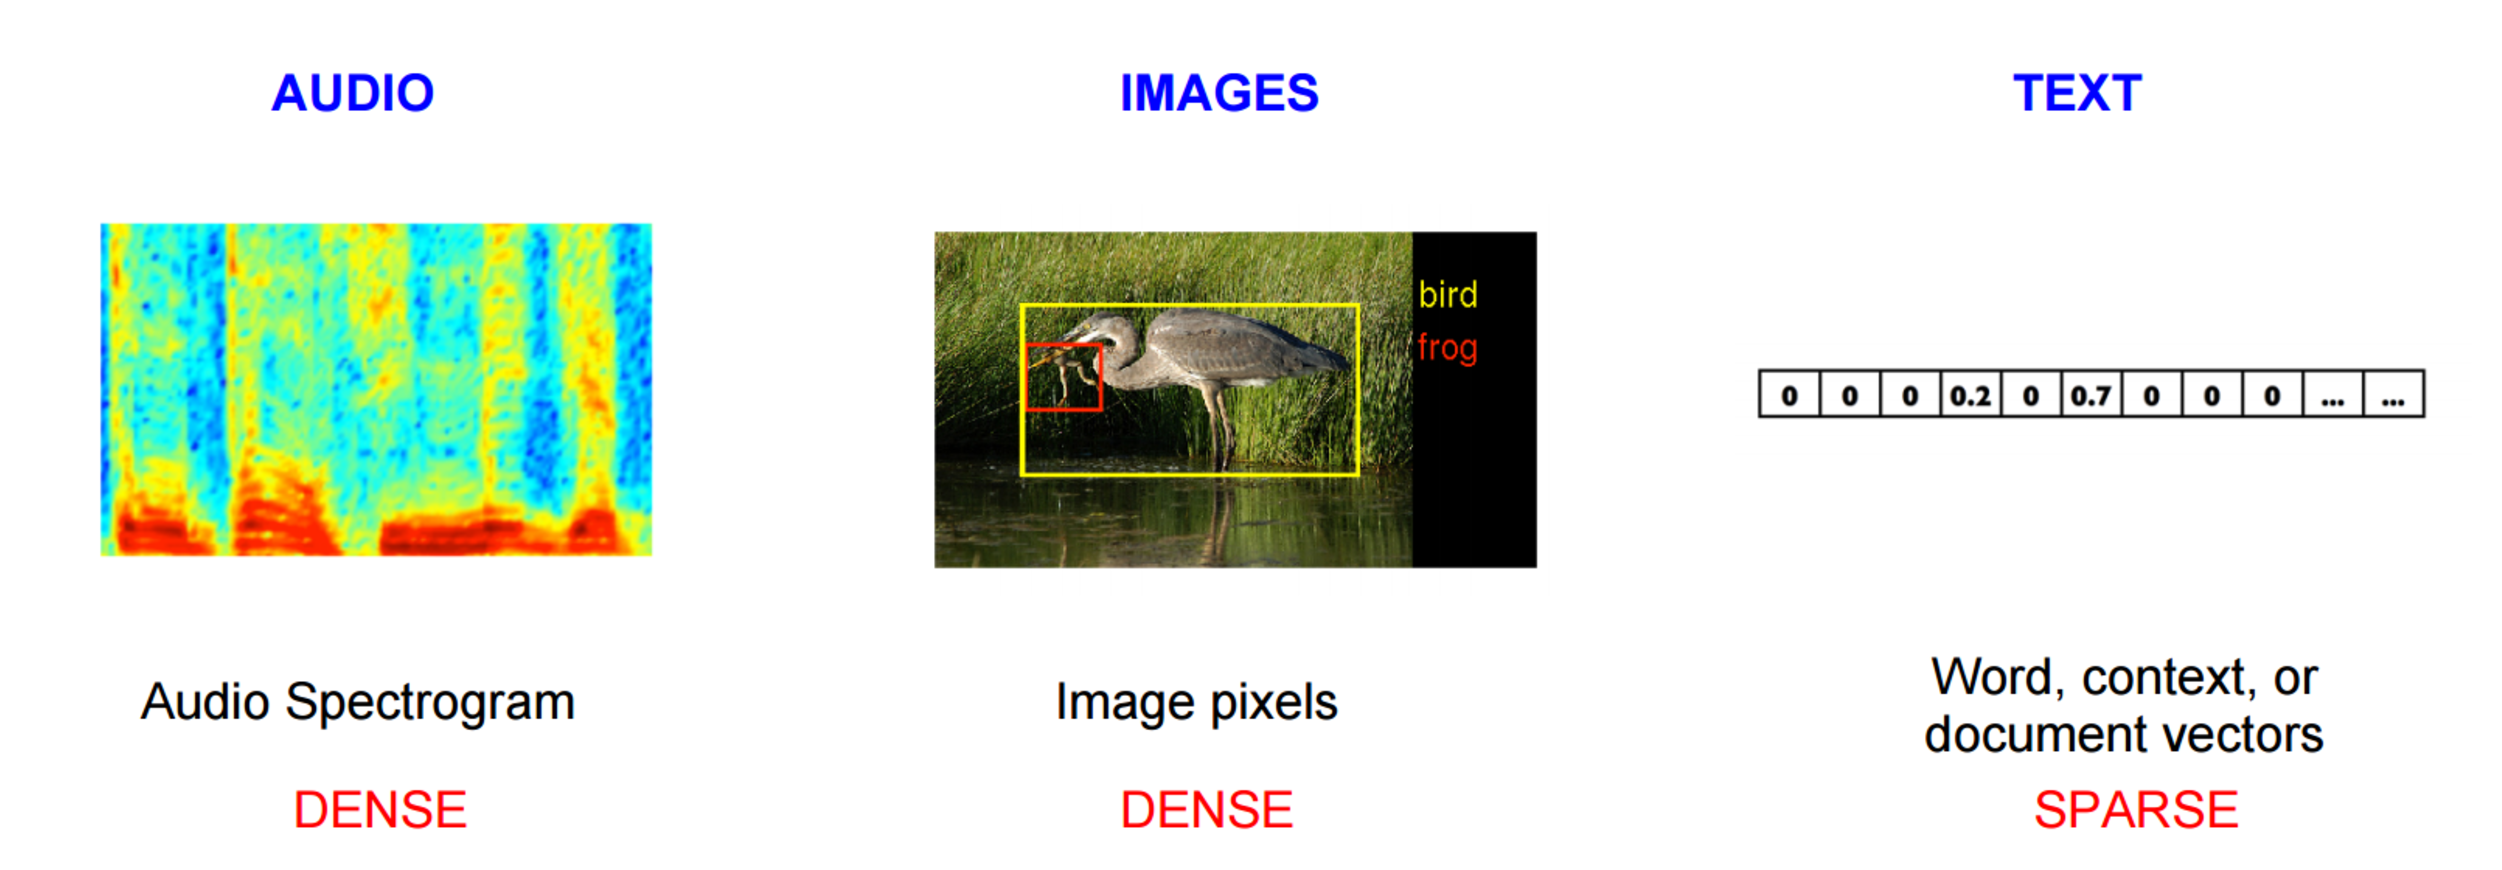
\includegraphics[width=\textwidth]{Images/comparison-text.png}
    \caption{Data sparsity in text \cite{comparison-text}}
    \label{comparison-text}
\end{figure}

Most learning algorithms rely on the local smoothness hypothesis, that is, similar training instances are spatially close. This hypothesis clearly doesn't hold with one-hot encoding as `dog' is as close as `tree' as it is with `cat'. Ideally, you would like to transform the word `dog' in a space so that it's closer to `cat' than it is to `tree'. That's exactly how word embedding works: every word is projected into a highly dimensional space that keep semantic relationships. Therefore, what the model has learned about dogs can be used when a cat is encountered. 

\subsection{Word2Vec overview}
The Word2Vec model by Mikolov et al. \cite{word2vec} is an efficient implementation of word embedding and works as follow:
Suppose you have a sentence: ``the ants in the garden". You can break that sentence in (context, target) pairs where the context are the words surrounding the target word. For example, if you take a context with a window of 1, you get the follow pairs: ([the, in], ants), ([ants, the], in), ([in, garden], the) [we omitted the pairs where the context wasn't of size 2]. You will then train a model to predict the target word given the context, and the weights of the model will give the word embedding (this will become clearer shortly). This model is called the Continuous Bag-of-Words model, and Word2Vec also comes in another flavor called the Skip-Gram model.

In the Skip-Gram model, you will predict the context given the target word, creating more pairs as for instance ([the, in], ants) are split into two training instances: (ants, the), (ants, in). The Continuous Bag-of-Words model smooth over the the distributional information by using the whole context, and works well on smaller datasets, but by breaking the (context, target) pair into more observations, the Skip-Gram model tends to perform better on larger datasets, and that's the model we will stick on from now on.

\subsection{Skip-Gram model}
The model is a neural network with one hidden layer and its objective is to predict the context word given the target. The input of the network will be a target word represented as a one-hot vector, of size say 10,000 (that's the vocabulary size) and the output will also be a vector of size 10,000 giving the probability distribution of the context word. Here is the architecture of the model:

\begin{figure}[H]
    \centering
    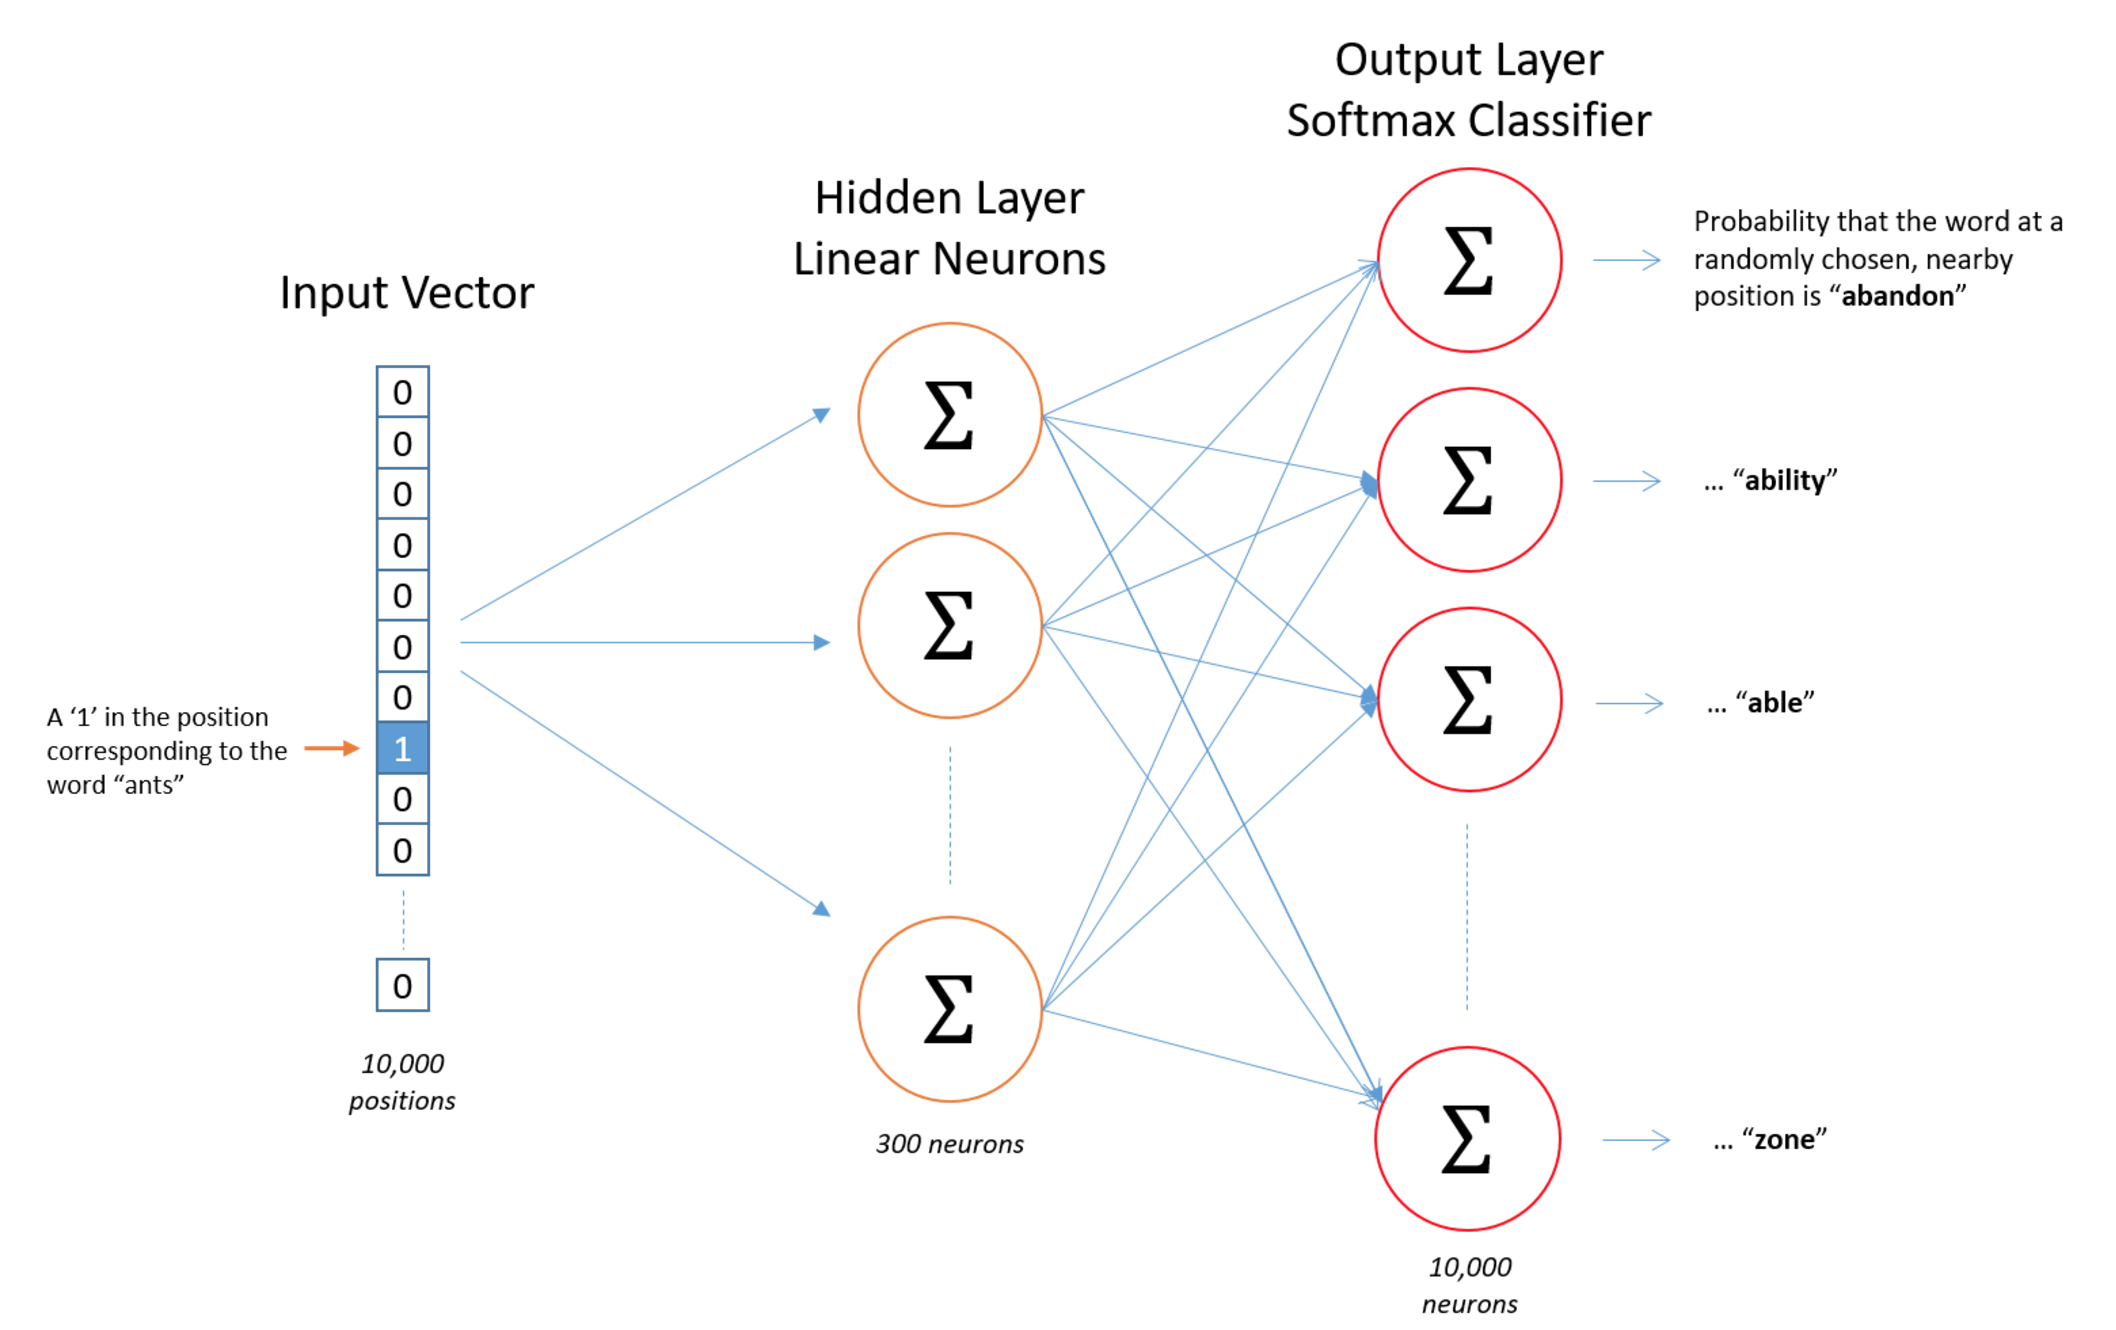
\includegraphics[width=\textwidth]{Images/word2vec-architecture.png}
    \caption{Skip-Gram model architecture \cite{word2vec-architecture}}
\end{figure}

There is no activation function in the hidden layer, but output neurons use softmax. The weights of the hidden layer matrix give the embedding as when you multiply a $1\times$10 000 one-hot vector with a 10 000$\times300$ matrix you select the row of size $1\times300$ corresponding to the high-dimensional representation of that word: 

\begin{figure}[H]
    \centering
    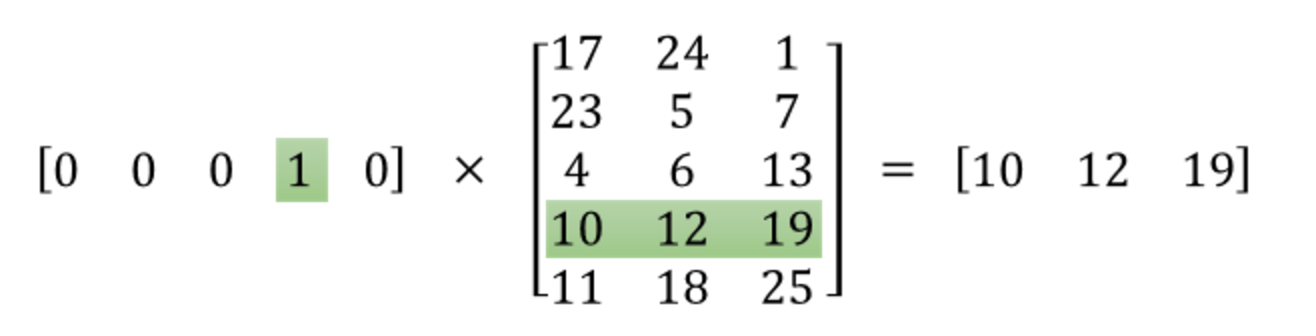
\includegraphics[width=0.8\textwidth]{Images/onehot-matrix.png}
    \caption{Where the embedding comes from \cite{word2vec-architecture}}
\end{figure}

To learn those weights, the network is minimising the cross-entropy loss given a (target word, context word) = $(w_t, c)$:
\begin{align}
    \text{J}_{\text{CE}}(w_t, c)   &=  -\text{log}P(w_t | c) \nonumber\\
    &= -\text{log}\{\text{softmax}(w_t, c)\}\nonumber\\
    &= -\text{log}\left(\frac{\text{exp}\{\text{score}(w_t, c)\}}{\sum_{\text{Word w' in Vocab}}\text{exp}\{\text{score}(w', c)\}} \right)
\end{align}

\subsection{Intuition}
In this model, two words that have similar contexts should output similar probability distribution. One way to produce that is to simply learn a similar word embedding for these two words. Therefore, words with similar context will have a similar vector representation which is exactly what we wanted.

Which words have similar contexts? Synonyms are a good example: `brave' and `fearless' are two words that must appear in similar contexts. The same applies for words that are related such as `physics' and `thermodynamics' or words with the same stem `apples' and 'apple'. 

\section{Training the model}
Training the network described above involves, with a vocabulary size of 10 000: 10 000$\times300$=3M parameters for the hidden layer and $300\times$10 000=3M for the output layer. In fact, the actual Word2Vec model contain 3M words, the number of parameters is thus 2$\times$3M$\times$300=1.8B. That's a huge neural network that will need a really large training set to train those parameters, which is not feasible without a few tweaks.

\subsection{Negative Sampling}
When training the model with gradient descent, each backward pass will update all the 1.8B parameters of the model. Negative sampling addresses this problem by only updating a fraction of the parameters.

For a given (target, context word) pair, we want the output of the model to be 1 on the context word and 0s for all the other words. With negative sampling, we'll instead randomly select a small subset of `negative samples' (a word we want the network to output a 0 for) to update the weights for. The paper by T. Mikolov et al. \cite{word2vec2} states that 5-20 negative samples for small datasets and 2-5 for large datasets achieve good results.

More specifically, the negative samples are selected using a `unigram distribution' with more frequent words more likely to be selected. The probability to select a word $w_i$ is simply its frequency $f_i$ to the power 3/4 (chosen empirically) divided by the sum of weights of all the other words:
\begin{equation}
P(w_i) = \frac{f_i^{3/4}}{\sum_{j=1}^V f_j^{3/4}}
\end{equation}

If we select 5 negative samples, then in the output layer those 5 words and the context word will be updated, and they each have 300 parameters (the embedding size) meaning that only 1800 parameters will be updated among the 0.9B parameters in the output layer, that's only 0.0002\% of the parameters.

In the hidden layer, only the weights of the input word (300 parameters) will be updated, but that's always the case regardless of negative sampling as the one-hot vector zero-out every weight in the hidden layer that does not belong to the input word.






